\PassOptionsToPackage{unicode=true}{hyperref} % options for packages loaded elsewhere
\PassOptionsToPackage{hyphens}{url}
\PassOptionsToPackage{dvipsnames,svgnames*,x11names*}{xcolor}
%
\documentclass[
  a4paper,
  twoside]{article}
\usepackage{lmodern}
\usepackage{amssymb,amsmath}
\usepackage{ifxetex,ifluatex}
\ifnum 0\ifxetex 1\fi\ifluatex 1\fi=0 % if pdftex
  \usepackage[T1]{fontenc}
  \usepackage[utf8]{inputenc}
  \usepackage{textcomp} % provides euro and other symbols
\else % if luatex or xelatex
  \usepackage{unicode-math}
  \defaultfontfeatures{Scale=MatchLowercase}
  \defaultfontfeatures[\rmfamily]{Ligatures=TeX,Scale=1}
  \setmainfont[]{Verdana}
\fi
% use upquote if available, for straight quotes in verbatim environments
\IfFileExists{upquote.sty}{\usepackage{upquote}}{}
\IfFileExists{microtype.sty}{% use microtype if available
  \usepackage[]{microtype}
  \UseMicrotypeSet[protrusion]{basicmath} % disable protrusion for tt fonts
}{}
\makeatletter
\@ifundefined{KOMAClassName}{% if non-KOMA class
  \IfFileExists{parskip.sty}{%
    \usepackage{parskip}
  }{% else
    \setlength{\parindent}{0pt}
    \setlength{\parskip}{6pt plus 2pt minus 1pt}}
}{% if KOMA class
  \KOMAoptions{parskip=half}}
\makeatother
\usepackage{xcolor}
\IfFileExists{xurl.sty}{\usepackage{xurl}}{} % add URL line breaks if available
\IfFileExists{bookmark.sty}{\usepackage{bookmark}}{\usepackage{hyperref}}
\hypersetup{
  pdftitle={Latex, YAML, RMarkdown},
  pdfauthor={Dortmunder Statistik},
  colorlinks=true,
  linkcolor=MidnightBlue,
  filecolor=Maroon,
  citecolor=Blue,
  urlcolor=MidnightBlue,
  breaklinks=true}
\urlstyle{same}  % don't use monospace font for urls
\usepackage[margin=1in]{geometry}
\usepackage{longtable,booktabs}
% Allow footnotes in longtable head/foot
\IfFileExists{footnotehyper.sty}{\usepackage{footnotehyper}}{\usepackage{footnote}}
\makesavenoteenv{longtable}
\usepackage{graphicx,grffile}
\makeatletter
\def\maxwidth{\ifdim\Gin@nat@width>\linewidth\linewidth\else\Gin@nat@width\fi}
\def\maxheight{\ifdim\Gin@nat@height>\textheight\textheight\else\Gin@nat@height\fi}
\makeatother
% Scale images if necessary, so that they will not overflow the page
% margins by default, and it is still possible to overwrite the defaults
% using explicit options in \includegraphics[width, height, ...]{}
\setkeys{Gin}{width=\maxwidth,height=\maxheight,keepaspectratio}
\setlength{\emergencystretch}{3em}  % prevent overfull lines
\providecommand{\tightlist}{%
  \setlength{\itemsep}{0pt}\setlength{\parskip}{0pt}}
\setcounter{secnumdepth}{5}
% Redefines (sub)paragraphs to behave more like sections
\ifx\paragraph\undefined\else
  \let\oldparagraph\paragraph
  \renewcommand{\paragraph}[1]{\oldparagraph{#1}\mbox{}}
\fi
\ifx\subparagraph\undefined\else
  \let\oldsubparagraph\subparagraph
  \renewcommand{\subparagraph}[1]{\oldsubparagraph{#1}\mbox{}}
\fi

% set default figure placement to htbp
\makeatletter
\def\fps@figure{htbp}
\makeatother

\setlength{\columnsep}{18pt}
\usepackage{multicol}
\newcommand{\hideFromPandoc}[1]{#1}
\hideFromPandoc{ \let\Begin\begin \let\End\end }
\definecolor{DoStat}{RGB}{4, 72, 145}
\definecolor{DoGray}{RGB}{33, 36, 39}
\usepackage{fancyhdr}
\pagestyle{fancy}
\fancyhf{}
\fancyhead[LE]{\itshape\nouppercase{\color{DoStat}\leftmark}}
\fancyhead[RO]{\itshape\nouppercase{\color{DoStat}\leftmark}}
\fancyfoot[LE]{\color{DoStat} \thepage \hspace{0.5cm} dortmunder\textbf{statistik}  • nr. 211 • RMarkdown, Latex und PDF • Erste Schritte}
\fancyfoot[RO]{\color{DoStat} dortmunder\textbf{statistik}  • nr. 211 • RMarkdown, Latex und PDF • Erste Schritte \hspace{0.5cm} \thepage}
\setlength{\headheight}{12.74066pt}
\usepackage{graphicx}
\usepackage[justification=justified,font=small,singlelinecheck=false]{caption}
\usepackage{color}
\DeclareCaptionFont{blue}{\color{DoStat}}
\captionsetup{labelfont={blue,bf}}
\AtBeginDocument{\let\maketitle\relax}
\newcommand\boldDoStat[1]{\textcolor{DoStat}{\textbf{#1}}}
\usepackage{booktabs}
\usepackage{longtable}
\usepackage{array}
\usepackage{multirow}
\usepackage{wrapfig}
\usepackage{float}
\usepackage{colortbl}
\usepackage{pdflscape}
\usepackage{tabu}
\usepackage{threeparttable}
\usepackage{threeparttablex}
\usepackage[normalem]{ulem}
\usepackage{makecell}
\usepackage{xcolor}

\title{Latex, YAML, RMarkdown}
\usepackage{etoolbox}
\makeatletter
\providecommand{\subtitle}[1]{% add subtitle to \maketitle
  \apptocmd{\@title}{\par {\large #1 \par}}{}{}
}
\makeatother
\subtitle{Options, packages and examples for PDF print}
\author{Dortmunder Statistik}
\date{}

\begin{document}
\maketitle

\renewcommand*\contentsname{Inhaltsverzeichnis}
{
\hypersetup{linkcolor=}
\setcounter{tocdepth}{4}
\tableofcontents
}
\newpage

\hypertarget{ziel}{%
\section{Ziel}\label{ziel}}

\textcolor{DoStat}{Heutiges Ziel:}

\begin{itemize}
\tightlist
\item
  erste Eindrücke von gelösten Layout-Problemstellungen in der Erstellung von RMarkdown/Latex basierten PDF Dokumenten
\item
  Plot Beispiele in 1- und 2 spaltigem Layout
\end{itemize}

\textcolor{DoStat}{Ziel des Prozesses:}

\begin{itemize}
\tightlist
\item
  Veröffentlichungen für Homepage oder interne Kooppartner, downloadbar auf der Seite der Dortmunder Statistik und ausdruckbar vor Ort
\item
  KEIN hochwertiges Printprodukt (bspw. Statistikatlas)
\item
  Plots basieren teilweise auf Daten aus dem Jahresbericht Bevölkerung 2019, teilweise auf frei verfügbare Daten
\item
  sie dienen lediglich als \textcolor{DoStat}{erste Beispiele} und bedürfen noch umfangreicher Formatierung für einen einheitliches Layout
\item
  Als Lückenfüller dient im Folgenden Lorem ipsum Text
\end{itemize}

\newpage

\begin {multicols}{2}

\vspace*{\textheight}

\columnbreak

\vspace*{12cm}

Die 2 spaltige Ausrichtung des Impressums kann über ``minipage'' gelöst werden, hat zeitlich nicht geklappt

\textcolor{DoStat}{\textbf{Impressum}}

\textbf{Herausgeber} \hspace{0.5cm} Stadt Dortmund, 3/Dez - Stabsstelle Dortmunder Statistik, 44122 Dortmund, 07/2019

\textbf{Redaktion} \hspace{0.5cm} Berthold Haermeyer (verantwortlich), Manfred Gabriel, Roland Scheebaum, Georg Schulte, Iwona Szargut

\textbf{Satz} \hspace{0.5cm} Rebecca Schluck

\textbf{Layout} \hspace{0.5cm} Gerd Schmedes, Gabak Solutions, Grafische Konstruktionen, Dortmund

\textbf{Kontakt} \hspace{0.5cm} InfoLine (0231) 50-22124, Telefax: (0231) 50-24777

\textbf{eMail} \hspace{0.5cm} \href{mailto:info.statistik@stadtdo.de}{\nolinkurl{info.statistik@stadtdo.de}}

\textbf{Internet} \hspace{0.5cm} www.statistik.dortmund.de

\textcolor{DoStat}{\textbf{Nachdruck, auch auszugsweise, mit Quellenangabe gestattet.}}

\end {multicols}

\newpage

\hypertarget{inhaltsverzeichnis}{%
\subsection{Inhaltsverzeichnis}\label{inhaltsverzeichnis}}

Das trockene Inhaltsverzeichis aus Seite 1 kann in Latex umfangreich formatiert werden (package: tocloft), beinhaltet aber viel Aufwand. Machbar, aber gut abzustimmen, im Hinblick auf die angefragten Produkten.

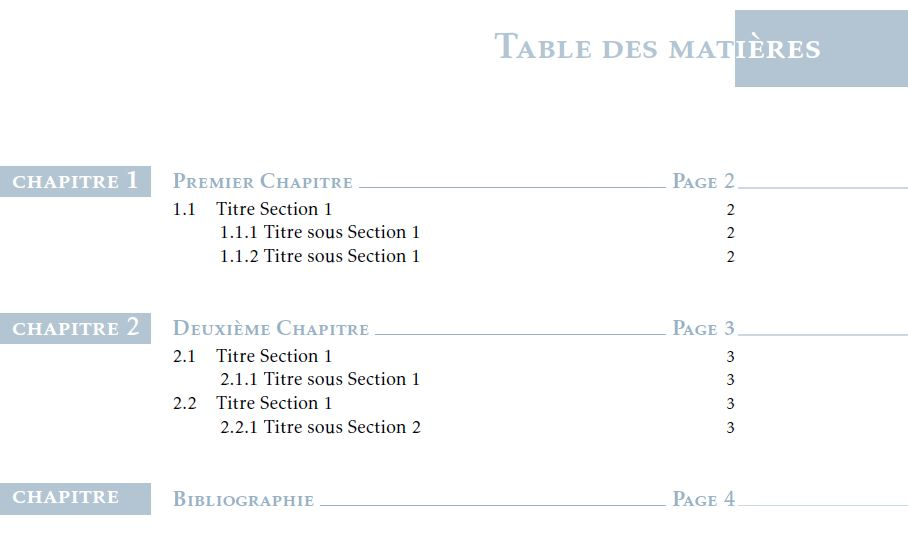
\includegraphics{B8obV.jpg}

\newpage

\hypertarget{und-2--spaltiges-textlayout}{%
\subsection{1- und 2- spaltiges Textlayout}\label{und-2--spaltiges-textlayout}}

Texte sind im 1- und 2 spaltigen Layout frei mit integrierten Plots kombinierbar. Ebenso sind Kopf- und Fußzeile anpassbar und wechseln von gerade auf ungerade Seite.

\begin {multicols}{2}

Lorem ipsum dolor sit amet, consetetur sadipscing elitr, sed diam nonumy eirmod tempor invidunt ut labore et dolore magna aliquyam erat, sed diam voluptua. At vero eos et accusam et justo duo dolores et ea rebum. Stet clita kasd gubergren, no sea takimata sanctus est Lorem ipsum dolor sit amet. Lorem ipsum dolor sit amet, consetetur sadipscing elitr, sed diam nonumy eirmod tempor invidunt ut labore et dolore magna aliquyam erat, sed diam voluptua. At vero eos et accusam et justo duo dolores et ea rebum. Stet clita kasd gubergren, no sea takimata sanctus est Lorem ipsum dolor sit amet.

\columnbreak

Lorem ipsum dolor sit amet, consetetur sadipscing elitr, sed diam nonumy eirmod tempor invidunt ut labore et dolore magna aliquyam erat, sed diam voluptua. At vero eos et accusam et justo duo dolores et ea rebum. Stet clita kasd gubergren, no sea takimata sanctus est Lorem ipsum dolor sit amet. Lorem ipsum dolor sit amet, consetetur sadipscing elitr, sed diam nonumy eirmod tempor invidunt ut labore et dolore magna aliquyam erat, sed diam voluptua. At vero eos et accusam et justo duo dolores et ea rebum. Stet clita kasd gubergren, no sea takimata sanctus est Lorem ipsum dolor sit amet.

\end {multicols}

\newpage

\hypertarget{mix-aus-plots-und-text}{%
\subsection{Mix aus Plots und Text}\label{mix-aus-plots-und-text}}

\begin {multicols}{2}

\begin{flushright}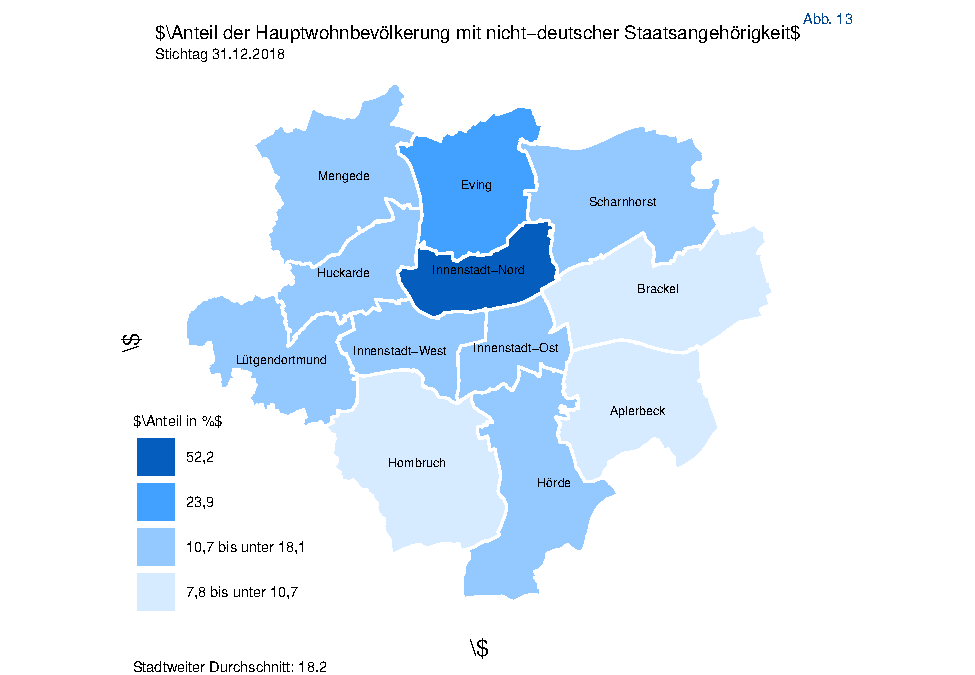
\includegraphics[width=1\linewidth]{2021-03-02_Beispiel_files/figure-latex/Plot map-1} \end{flushright}

Lorem ipsum dolor sit amet, consetetur sadipscing elitr, sed diam nonumy eirmod tempor invidunt ut labore et dolore magna aliquyam erat, sed diam voluptua. At vero eos et accusam et justo duo dolores et ea rebum. Stet clita kasd gubergren, no sea takimata sanctus est Lorem ipsum dolor sit amet. Lorem ipsum dolor sit amet, consetetur sadipscing elitr, sed diam nonumy eirmod tempor invidunt ut labore et dolore magna aliquyam erat, sed diam voluptua. At vero eos et accusam et justo duo dolores et ea rebum. Stet clita kasd gubergren, no sea takimata sanctus est Lorem ipsum dolor sit amet.

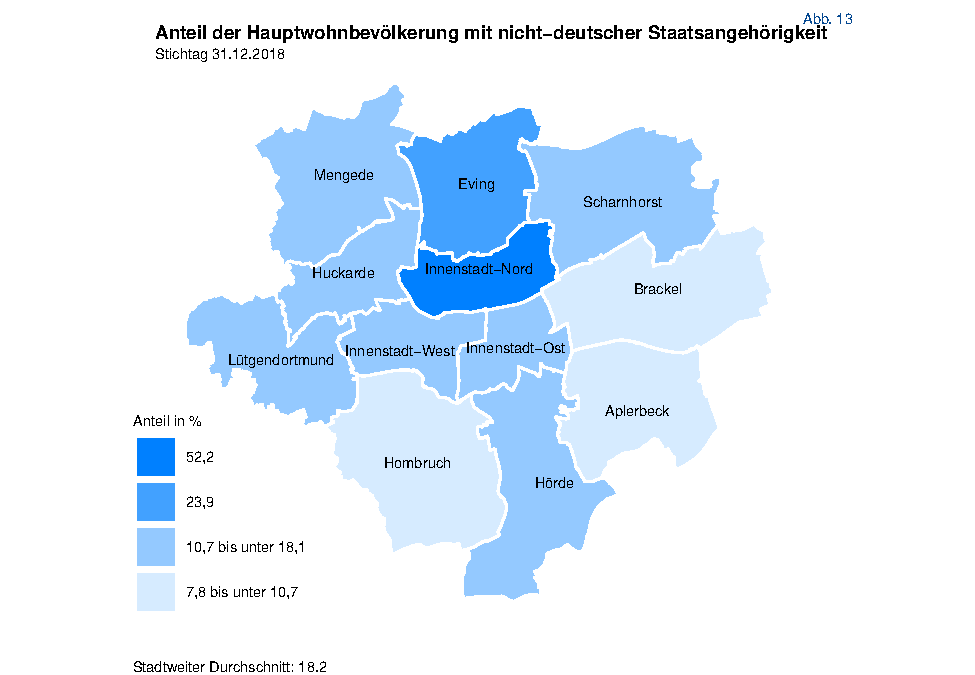
\includegraphics[width=1\linewidth]{2021-03-02_Beispiel_files/figure-latex/unnamed-chunk-1-1}

\columnbreak

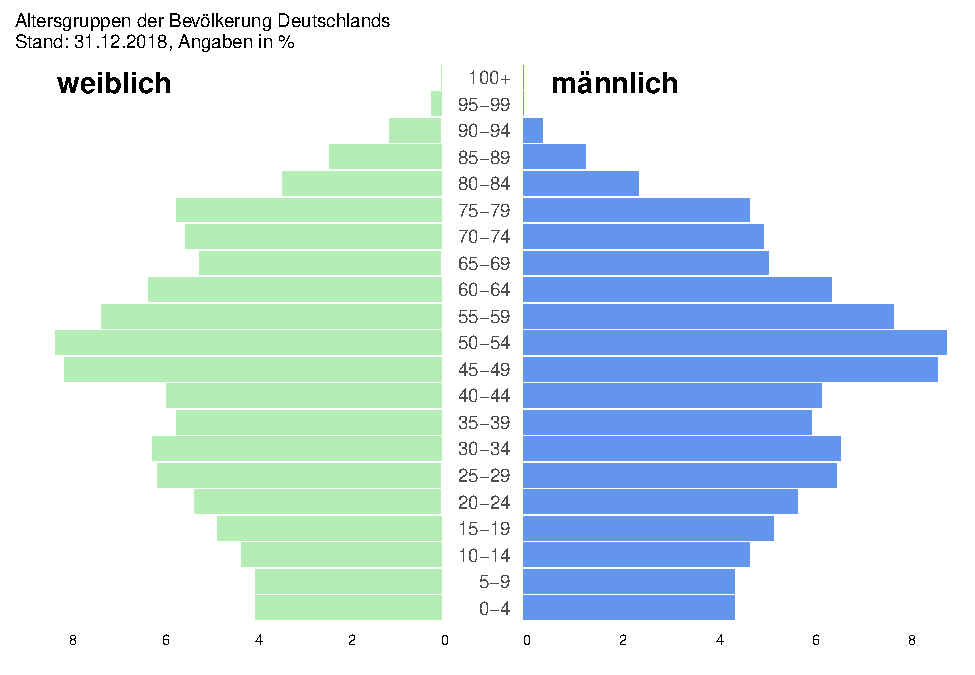
\includegraphics[width=1\linewidth]{2021-03-02_Beispiel_files/figure-latex/plot Pyramide 2-spaltig-1}

Lorem ipsum dolor sit amet, consetetur sadipscing elitr, sed diam nonumy eirmod tempor invidunt ut labore et dolore magna aliquyam erat, sed diam voluptua. At vero eos et accusam et justo duo dolores et ea rebum. Stet clita kasd gubergren, no sea takimata sanctus est Lorem ipsum dolor sit amet. Lorem ipsum dolor sit amet, consetetur sadipscing elitr, sed diam nonumy eirmod tempor invidunt ut labore et dolore magna aliquyam erat, sed diam voluptua. At vero eos et accusam et justo duo dolores et ea rebum. Stet clita kasd gubergren, no sea takimata sanctus est Lorem ipsum dolor sit amet.

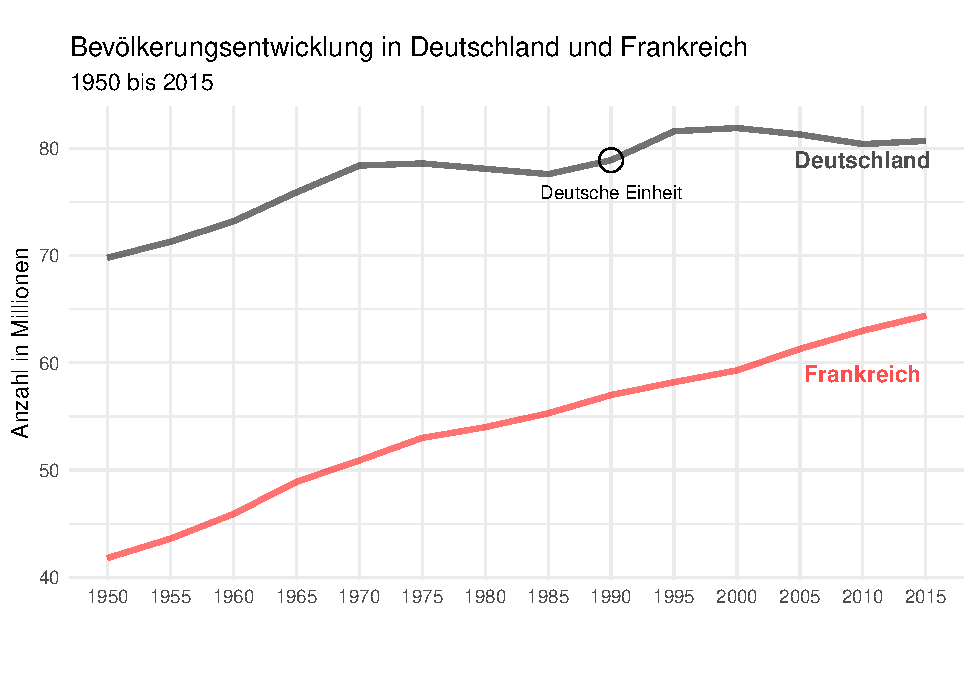
\includegraphics[width=1\linewidth]{2021-03-02_Beispiel_files/figure-latex/unnamed-chunk-2-1}

\end {multicols}

\newpage

\hypertarget{plots-1-spaltig}{%
\subsection{Plots 1 spaltig}\label{plots-1-spaltig}}

Hier eine Ansicht in maximaler Größe

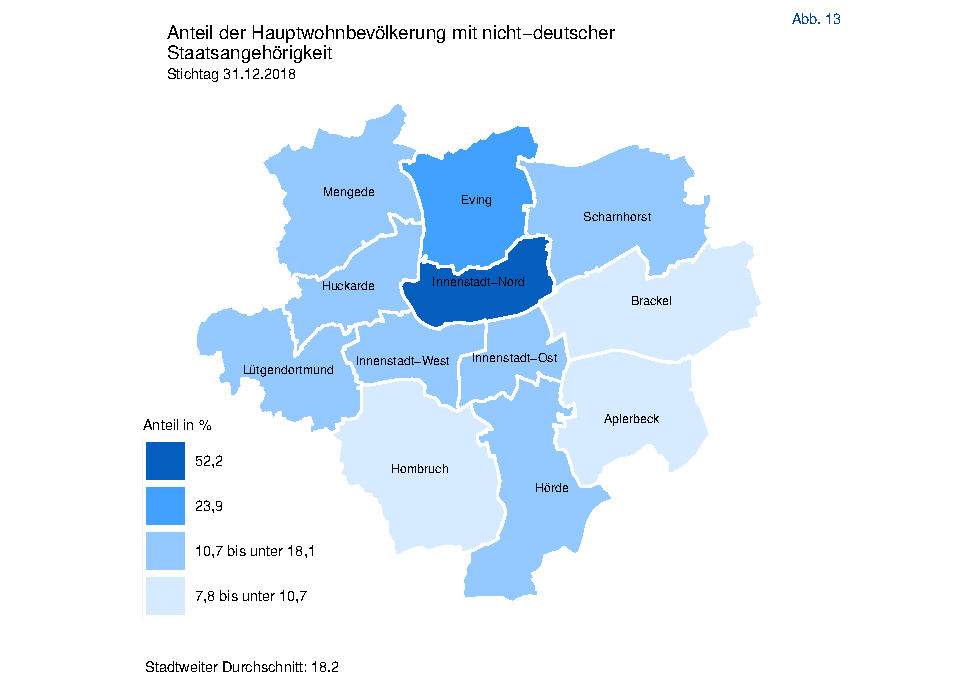
\includegraphics[width=1\linewidth]{2021-03-02_Beispiel_files/figure-latex/Plot map 1 spaltig-1}

\vspace{5mm}

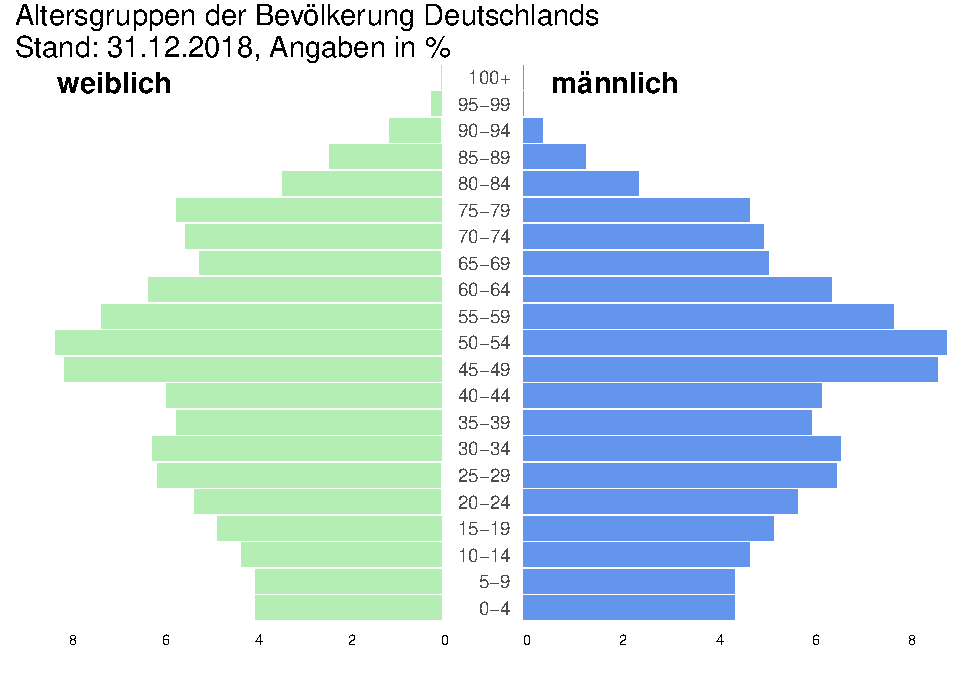
\includegraphics[width=1\linewidth]{2021-03-02_Beispiel_files/figure-latex/plot Pyramide 1 spaltig-1}

\newpage

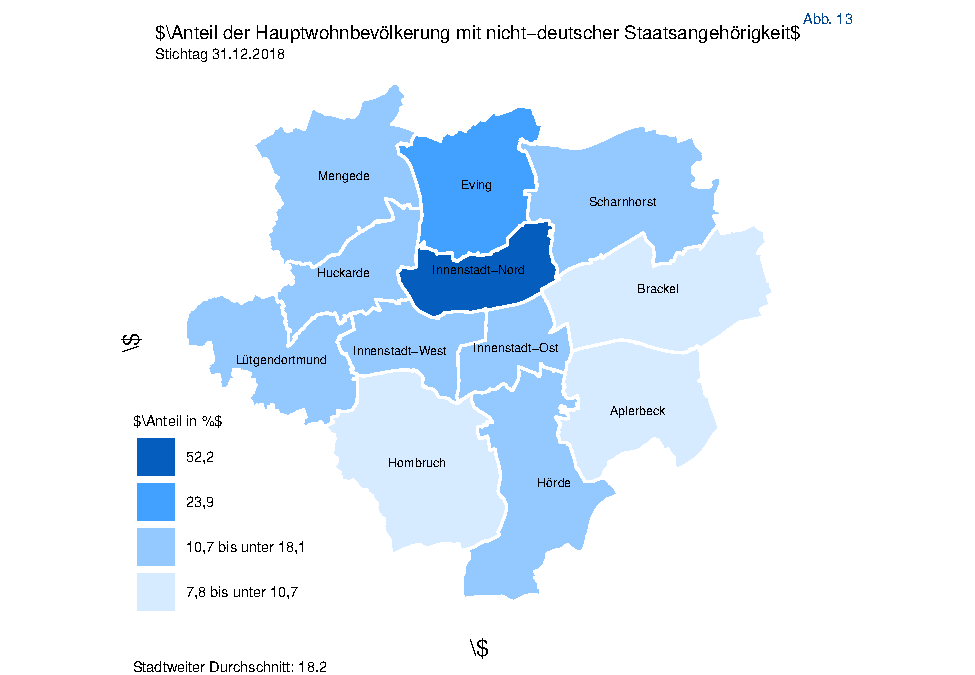
\includegraphics[width=1\linewidth]{2021-03-02_Beispiel_files/figure-latex/unnamed-chunk-3-1}

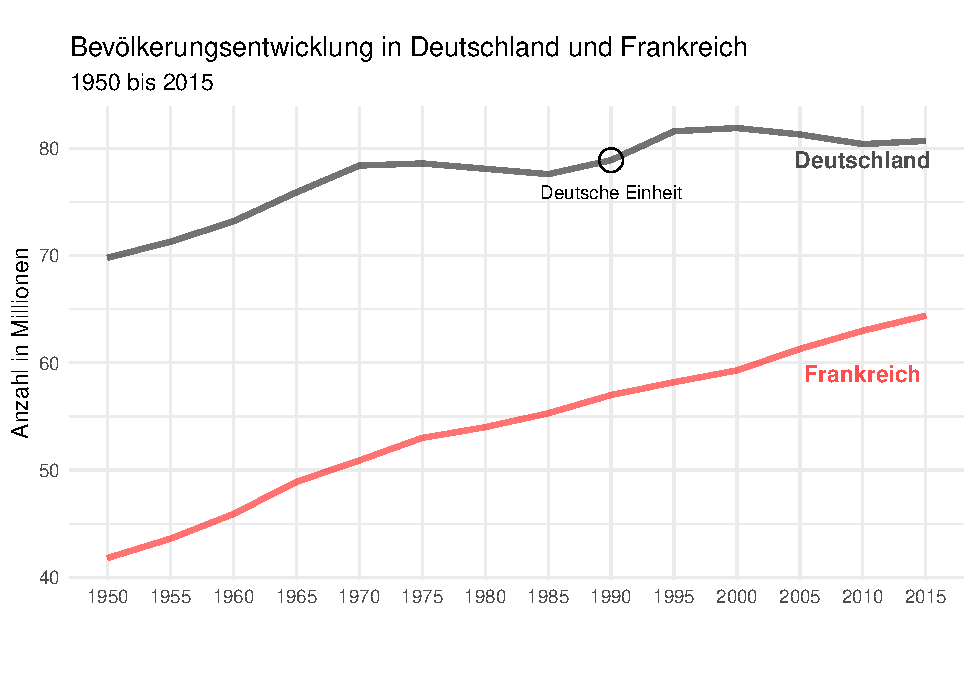
\includegraphics[width=1\linewidth]{2021-03-02_Beispiel_files/figure-latex/unnamed-chunk-4-1}

\newpage

\hypertarget{tabelle-ganzseitig}{%
\subsection{Tabelle Ganzseitig}\label{tabelle-ganzseitig}}

\begin{table}[!h]

\caption{\label{tab:kable}Stadtbezirk Innenstadt-West: Bevölkerung im Zeitvergleich 2013 bis 2018}
\centering
\resizebox{\linewidth}{!}{
\begin{threeparttable}
\begin{tabular}[t]{>{}l>{}r>{}r>{}r>{}r>{}r>{}r>{}r>{}r}
\toprule
\multicolumn{1}{c}{\textcolor{DoGray}{ }} & \multicolumn{2}{c}{\textcolor{DoGray}{2013}} & \multicolumn{2}{c}{\textcolor{DoGray}{2017}} & \multicolumn{2}{c}{\textcolor{DoGray}{2018}} & \multicolumn{1}{c}{\textcolor{DoGray}{2018 / 2013}} & \multicolumn{1}{c}{\textcolor{DoGray}{2018 / 2017}} \\
\cmidrule(l{3pt}r{3pt}){2-3} \cmidrule(l{3pt}r{3pt}){4-5} \cmidrule(l{3pt}r{3pt}){6-7} \cmidrule(l{3pt}r{3pt}){8-8} \cmidrule(l{3pt}r{3pt}){9-9}
\textcolor{DoGray}{Stadtbezirk Innenstadt-West} & \textcolor{DoGray}{Anzahl} & \textcolor{DoGray}{\makecell[c]{in \% der \\HWB}} & \textcolor{DoGray}{Anzahl} & \textcolor{DoGray}{\makecell[c]{in \% der \\HWB}} & \textcolor{DoGray}{Anzahl} & \textcolor{DoGray}{\makecell[c]{in \% der \\HWB}} & \textcolor{DoGray}{\makecell[c]{Anzahl\\}} & \textcolor{DoGray}{\makecell[c]{Anzahl\\}}\\
\midrule
\addlinespace[0.3em]
\multicolumn{9}{l}{\textcolor[HTML]{044891}{Hauptwohnbevölkerung (HWB)}}\\
\hspace{1em}\hspace{1em}\textcolor{DoGray}{Insgesamt} & \textcolor{DoGray}{52031} & \textcolor{DoGray}{100.0} & \textcolor{DoGray}{53323} & \textcolor{DoGray}{100.0} & \textcolor{DoGray}{52970} & \textcolor{DoGray}{100.0} & \textcolor{DoGray}{939} & \textcolor{DoGray}{-353}\\
\addlinespace[0.3em]
\multicolumn{9}{l}{\textcolor[HTML]{044891}{Bevölkerung nach Geschlecht}}\\
\hspace{1em}\hspace{1em}\textcolor{DoGray}{Männlich} & \textcolor{DoGray}{25739} & \textcolor{DoGray}{49.5} & \textcolor{DoGray}{26613} & \textcolor{DoGray}{49.9} & \textcolor{DoGray}{26441} & \textcolor{DoGray}{49.9} & \textcolor{DoGray}{702} & \textcolor{DoGray}{-172}\\
\hspace{1em}\hspace{1em}\textcolor{DoGray}{Weiblich} & \textcolor{DoGray}{26292} & \textcolor{DoGray}{50.5} & \textcolor{DoGray}{26710} & \textcolor{DoGray}{50.1} & \textcolor{DoGray}{26529} & \textcolor{DoGray}{50.1} & \textcolor{DoGray}{237} & \textcolor{DoGray}{-181}\\
\addlinespace[0.3em]
\multicolumn{9}{l}{\textcolor[HTML]{044891}{Bevölkerung nach Migrationshintergrund}}\\
\hspace{1em}\hspace{1em}\textcolor{DoGray}{Deutsch} & \textcolor{DoGray}{44023} & \textcolor{DoGray}{84.6} & \textcolor{DoGray}{43702} & \textcolor{DoGray}{82.0} & \textcolor{DoGray}{43362} & \textcolor{DoGray}{81.9} & \textcolor{DoGray}{-661} & \textcolor{DoGray}{-340}\\
\hspace{1em}\hspace{2em}\textcolor{DoGray}{dav. ohne Migrationshintergrund} & \textcolor{DoGray}{35589} & \textcolor{DoGray}{68.4} & \textcolor{DoGray}{35419} & \textcolor{DoGray}{66.4} & \textcolor{DoGray}{34802} & \textcolor{DoGray}{65.7} & \textcolor{DoGray}{-$^{4}$} & \textcolor{DoGray}{-617}\\
\hspace{1em}\hspace{2em}\textcolor{DoGray}{dav. mit Migrationshintergrund} & \textcolor{DoGray}{8434} & \textcolor{DoGray}{16.2} & \textcolor{DoGray}{8283} & \textcolor{DoGray}{15.5} & \textcolor{DoGray}{8560} & \textcolor{DoGray}{16.2} & \textcolor{DoGray}{-$^{4}$} & \textcolor{DoGray}{277}\\
\hspace{1em}\hspace{1em}\textcolor{DoGray}{Nichtdeutsch (1. Staatsangehörigkeit)} & \textcolor{DoGray}{8008} & \textcolor{DoGray}{15.4} & \textcolor{DoGray}{9621} & \textcolor{DoGray}{18.0} & \textcolor{DoGray}{9608} & \textcolor{DoGray}{18.1} & \textcolor{DoGray}{1600} & \textcolor{DoGray}{-13}\\
\addlinespace[0.3em]
\multicolumn{9}{l}{\textcolor[HTML]{044891}{Bevölkerung nach Altersgruppen}}\\
\hspace{1em}\hspace{1em}\textcolor{DoGray}{0 bis unter 3 Jahre} & \textcolor{DoGray}{1238} & \textcolor{DoGray}{2.4} & \textcolor{DoGray}{1356} & \textcolor{DoGray}{2.5} & \textcolor{DoGray}{1313} & \textcolor{DoGray}{2.5} & \textcolor{DoGray}{75} & \textcolor{DoGray}{-43}\\
\hspace{1em}\hspace{1em}\textcolor{DoGray}{3 bis unter 6 Jahre} & \textcolor{DoGray}{1102} & \textcolor{DoGray}{2.1} & \textcolor{DoGray}{1136} & \textcolor{DoGray}{2.1} & \textcolor{DoGray}{1122} & \textcolor{DoGray}{2.1} & \textcolor{DoGray}{20} & \textcolor{DoGray}{-14}\\
\hspace{1em}\hspace{1em}\textcolor{DoGray}{6 bis unter 18 Jahre} & \textcolor{DoGray}{4123} & \textcolor{DoGray}{7.9} & \textcolor{DoGray}{4172} & \textcolor{DoGray}{7.8} & \textcolor{DoGray}{4140} & \textcolor{DoGray}{7.8} & \textcolor{DoGray}{17} & \textcolor{DoGray}{-32}\\
\hspace{1em}\hspace{1em}\textcolor{DoGray}{18 bis unter 25 Jahre} & \textcolor{DoGray}{5729} & \textcolor{DoGray}{11.0} & \textcolor{DoGray}{5773} & \textcolor{DoGray}{10.8} & \textcolor{DoGray}{5692} & \textcolor{DoGray}{10.7} & \textcolor{DoGray}{-37} & \textcolor{DoGray}{-81}\\
\hspace{1em}\hspace{1em}\textcolor{DoGray}{25 bis unter 35 Jahre} & \textcolor{DoGray}{10667} & \textcolor{DoGray}{20.5} & \textcolor{DoGray}{11713} & \textcolor{DoGray}{22.0} & \textcolor{DoGray}{11554} & \textcolor{DoGray}{21.8} & \textcolor{DoGray}{887} & \textcolor{DoGray}{-159}\\
\hspace{1em}\hspace{1em}\textcolor{DoGray}{35 bis unter 50 Jahre} & \textcolor{DoGray}{11095} & \textcolor{DoGray}{21.3} & \textcolor{DoGray}{10331} & \textcolor{DoGray}{19.4} & \textcolor{DoGray}{10203} & \textcolor{DoGray}{19.3} & \textcolor{DoGray}{-892} & \textcolor{DoGray}{-128}\\
\hspace{1em}\hspace{1em}\textcolor{DoGray}{50 bis unter 65 Jahre} & \textcolor{DoGray}{9259} & \textcolor{DoGray}{17.8} & \textcolor{DoGray}{9927} & \textcolor{DoGray}{18.6} & \textcolor{DoGray}{9965} & \textcolor{DoGray}{18.8} & \textcolor{DoGray}{706} & \textcolor{DoGray}{38}\\
\hspace{1em}\hspace{1em}\textcolor{DoGray}{65 bis unter 80 Jahre} & \textcolor{DoGray}{6294} & \textcolor{DoGray}{12.1} & \textcolor{DoGray}{6215} & \textcolor{DoGray}{11.7} & \textcolor{DoGray}{6180} & \textcolor{DoGray}{11.7} & \textcolor{DoGray}{-114} & \textcolor{DoGray}{-35}\\
\hspace{1em}\hspace{1em}\textcolor{DoGray}{80 Jahre und älter} & \textcolor{DoGray}{2524} & \textcolor{DoGray}{4.9} & \textcolor{DoGray}{2700} & \textcolor{DoGray}{5.1} & \textcolor{DoGray}{2801} & \textcolor{DoGray}{5.3} & \textcolor{DoGray}{277} & \textcolor{DoGray}{101}\\
\addlinespace[0.3em]
\multicolumn{9}{l}{\textcolor[HTML]{044891}{Bevölkerung nach Familienstand}}\\
\hspace{1em}\hspace{1em}\textcolor{DoGray}{Ledig} & \textcolor{DoGray}{27380} & \textcolor{DoGray}{52.6} & \textcolor{DoGray}{28898} & \textcolor{DoGray}{54.2} & \textcolor{DoGray}{28697} & \textcolor{DoGray}{54.2} & \textcolor{DoGray}{1317} & \textcolor{DoGray}{-201}\\
\hspace{1em}\hspace{1em}\textcolor{DoGray}{Verheiratet} & \textcolor{DoGray}{16667} & \textcolor{DoGray}{32.0} & \textcolor{DoGray}{16426} & \textcolor{DoGray}{30.8} & \textcolor{DoGray}{16319} & \textcolor{DoGray}{30.8} & \textcolor{DoGray}{-348} & \textcolor{DoGray}{-107}\\
\hspace{1em}\hspace{1em}\textcolor{DoGray}{Verwitwet} & \textcolor{DoGray}{3266} & \textcolor{DoGray}{6.3} & \textcolor{DoGray}{3107} & \textcolor{DoGray}{5.8} & \textcolor{DoGray}{3039} & \textcolor{DoGray}{5.7} & \textcolor{DoGray}{-227} & \textcolor{DoGray}{-68}\\
\hspace{1em}\hspace{1em}\textcolor{DoGray}{Geschieden} & \textcolor{DoGray}{4458} & \textcolor{DoGray}{8.6} & \textcolor{DoGray}{4358} & \textcolor{DoGray}{8.2} & \textcolor{DoGray}{4290} & \textcolor{DoGray}{8.1} & \textcolor{DoGray}{-168} & \textcolor{DoGray}{-68}\\
\hspace{1em}\hspace{1em}\textcolor{DoGray}{Sonstige$^{1}$} & \textcolor{DoGray}{260} & \textcolor{DoGray}{0.5} & \textcolor{DoGray}{534} & \textcolor{DoGray}{1.0} & \textcolor{DoGray}{625} & \textcolor{DoGray}{1.2} & \textcolor{DoGray}{365} & \textcolor{DoGray}{91}\\
\addlinespace[0.3em]
\multicolumn{9}{l}{\textcolor[HTML]{044891}{Bevölkerung nach Konfession}}\\
\hspace{1em}\hspace{1em}\textcolor{DoGray}{Evangelisch} & \textcolor{DoGray}{13735} & \textcolor{DoGray}{26.4} & \textcolor{DoGray}{12829} & \textcolor{DoGray}{24.1} & \textcolor{DoGray}{12549} & \textcolor{DoGray}{23.7} & \textcolor{DoGray}{-1186} & \textcolor{DoGray}{-280}\\
\hspace{1em}\hspace{1em}\textcolor{DoGray}{Römisch-katholisch} & \textcolor{DoGray}{14848} & \textcolor{DoGray}{28.5} & \textcolor{DoGray}{14298} & \textcolor{DoGray}{26.8} & \textcolor{DoGray}{14017} & \textcolor{DoGray}{26.5} & \textcolor{DoGray}{-831} & \textcolor{DoGray}{-281}\\
\hspace{1em}\hspace{1em}\textcolor{DoGray}{Sonstige$^{1}$, ohne Angabe, keine} & \textcolor{DoGray}{23448} & \textcolor{DoGray}{45.1} & \textcolor{DoGray}{26196} & \textcolor{DoGray}{49.1} & \textcolor{DoGray}{26404} & \textcolor{DoGray}{49.8} & \textcolor{DoGray}{2956} & \textcolor{DoGray}{208}\\
\addlinespace[0.3em]
\multicolumn{9}{l}{\textcolor[HTML]{044891}{Bevölkerung mit Nebenwohnsitz}}\\
\hspace{1em}\hspace{1em}\textcolor{DoGray}{Insgesamt} & \textcolor{DoGray}{1060} & \textcolor{DoGray}{2.0} & \textcolor{DoGray}{1014} & \textcolor{DoGray}{1.9} & \textcolor{DoGray}{969} & \textcolor{DoGray}{1.8} & \textcolor{DoGray}{-91} & \textcolor{DoGray}{-45}\\
\addlinespace[0.3em]
\multicolumn{9}{l}{\textcolor[HTML]{044891}{Bevölkerung nach Haushalten}}\\
\hspace{1em}\hspace{1em}\textcolor{DoGray}{Einpersonenhaushalte} & \textcolor{DoGray}{19985} & \textcolor{DoGray}{38.4} & \textcolor{DoGray}{20393} & \textcolor{DoGray}{38.2} & \textcolor{DoGray}{20501} & \textcolor{DoGray}{38.7} & \textcolor{DoGray}{-$^{4}$} & \textcolor{DoGray}{108}\\
\hspace{1em}\hspace{1em}\textcolor{DoGray}{(Ehe-)Paare ohne Kind(er)} & \textcolor{DoGray}{14881} & \textcolor{DoGray}{28.6} & \textcolor{DoGray}{15027} & \textcolor{DoGray}{28.2} & \textcolor{DoGray}{15027} & \textcolor{DoGray}{28.4} & \textcolor{DoGray}{-$^{4}$} & \textcolor{DoGray}{0}\\
\hspace{1em}\hspace{1em}\textcolor{DoGray}{(Ehe-)Paare mit Kind(ern)} & \textcolor{DoGray}{11209} & \textcolor{DoGray}{21.5} & \textcolor{DoGray}{11410} & \textcolor{DoGray}{21.4} & \textcolor{DoGray}{11193} & \textcolor{DoGray}{21.1} & \textcolor{DoGray}{-$^{4}$} & \textcolor{DoGray}{-217}\\
\hspace{1em}\hspace{1em}\textcolor{DoGray}{Alleinerziehende Haushalte} & \textcolor{DoGray}{3147} & \textcolor{DoGray}{6.0} & \textcolor{DoGray}{2926} & \textcolor{DoGray}{5.5} & \textcolor{DoGray}{2979} & \textcolor{DoGray}{5.6} & \textcolor{DoGray}{-$^{4}$} & \textcolor{DoGray}{53}\\
\hspace{1em}\hspace{1em}\textcolor{DoGray}{Sonstige$^{1}$ Mehrpersonenhaushalte} & \textcolor{DoGray}{2809} & \textcolor{DoGray}{5.4} & \textcolor{DoGray}{2836} & \textcolor{DoGray}{5.3} & \textcolor{DoGray}{2770} & \textcolor{DoGray}{5.2} & \textcolor{DoGray}{-$^{4}$} & \textcolor{DoGray}{-66}\\
\hspace{1em}\hspace{1em}\textcolor{DoGray}{Bevölkerung in Haushalten insgesamt$^{3}$} & \textcolor{DoGray}{52031} & \textcolor{DoGray}{100.0} & \textcolor{DoGray}{52592} & \textcolor{DoGray}{98.6} & \textcolor{DoGray}{52470} & \textcolor{DoGray}{99.1} & \textcolor{DoGray}{-$^{4}$} & \textcolor{DoGray}{-122}\\
\addlinespace[0.3em]
\multicolumn{9}{l}{\textcolor[HTML]{044891}{Bevölkerung nach Statistischen Bezirken}}\\
\hspace{1em}\hspace{1em}\textcolor{DoGray}{000-City} & \textcolor{DoGray}{9337} & \textcolor{DoGray}{17.9} & \textcolor{DoGray}{9687} & \textcolor{DoGray}{18.2} & \textcolor{DoGray}{9707} & \textcolor{DoGray}{18.3} & \textcolor{DoGray}{370} & \textcolor{DoGray}{20}\\
\hspace{1em}\hspace{1em}\textcolor{DoGray}{010-Westfalenhalle} & \textcolor{DoGray}{15517} & \textcolor{DoGray}{29.8} & \textcolor{DoGray}{15828} & \textcolor{DoGray}{29.7} & \textcolor{DoGray}{15863} & \textcolor{DoGray}{29.9} & \textcolor{DoGray}{346} & \textcolor{DoGray}{35}\\
\hspace{1em}\hspace{1em}\textcolor{DoGray}{020-Dorstfelder Brücke} & \textcolor{DoGray}{11882} & \textcolor{DoGray}{22.8} & \textcolor{DoGray}{12458} & \textcolor{DoGray}{23.4} & \textcolor{DoGray}{12362} & \textcolor{DoGray}{23.3} & \textcolor{DoGray}{480} & \textcolor{DoGray}{-96}\\
\hspace{1em}\hspace{1em}\textcolor{DoGray}{030-Dorstfeld} & \textcolor{DoGray}{15295} & \textcolor{DoGray}{29.4} & \textcolor{DoGray}{15350} & \textcolor{DoGray}{28.8} & \textcolor{DoGray}{15038} & \textcolor{DoGray}{28.4} & \textcolor{DoGray}{-257} & \textcolor{DoGray}{-312}\\
\bottomrule
\end{tabular}
\begin{tablenotes}
\small
\item[1] \textcolor{DoGray}{Hierzu zählen Lebenspartnerschaft, Lebenspartnerschaft aufgehoben, Lebenspartner verstorben und unbekannt.}
\item[2] \textcolor{DoGray}{Sonstige Mehrpersonenhaushalte ohne Paare und ohne Kinder.}
\item[3] \textcolor{DoGray}{Seit 2016 werden durch methodische Verbesserungen in der Haushaltegenerierung Personen in Gemeinschaftsunterkünften ausgeschlossen, weshalb die Bevölkerung in Haushalten insgesamt ab 2016 unter 100 \% der HWB liegt. Die Differenz sind die Personen in Gemeinschaftsunterkünften.}
\item[4] \textcolor{DoGray}{Durch methodische Verbesserungen (seit 2016) in der Generierung der Daten zum Migrationshintergrund und zu den Haushalten, sind die Daten für einen Zeitvergleich nicht geeignet.}
\end{tablenotes}
\end{threeparttable}}
\end{table}

\newpage

\end{document}
